A promotional video was created to market the project. The video needed to be approximately two minutes and the purpose of it was to show off the features of the platform.
To capture the audience attention while still describing the platform in under two minutes proved to be a challenge. A storyboard was constructed to plan and make sure the video would have clear purpose and goal.

% This is in Swedish!
%\begin{figure}[h]
%    \centering
%    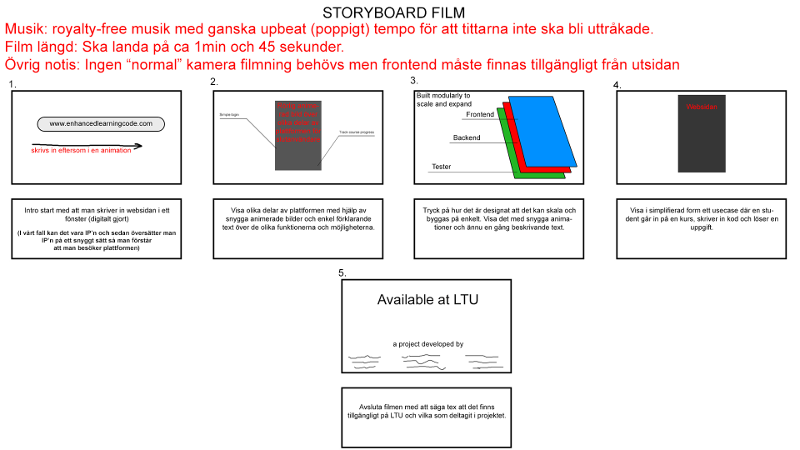
\includegraphics[width=.8\linewidth]{storboard-promo_resized.png}
%    \caption{Image of the storyboard for the promotional video}
%\end{figure}

\begin{figure}[ht]
    \centering

    \begin{subfigure}{.3\linewidth}
    \centering
    
\includegraphics[width=\linewidth]{img/video_1.png}
    \end{subfigure}
    \hfill
    \begin{subfigure}{.3\linewidth}
    \centering
    
\includegraphics[width=\linewidth]{img/video_2.png}
    \end{subfigure}
    \hfill
    \begin{subfigure}{.3\linewidth}
    \centering
    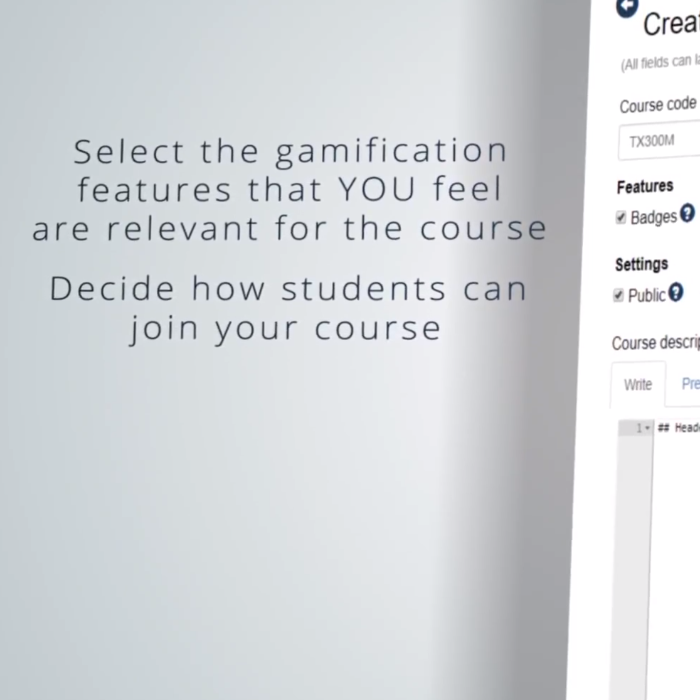
\includegraphics[width=\linewidth]{img/video_3.png}
    \end{subfigure}

    \caption{Sample images from the promotional video.}
\end{figure}

After the storyboard was completed, a lot of time was spent finding the right type of royalty-free music. Once a suitable song was found, the video recording of the system was done. Pictures of every page of the site was also snapped. However, once most of the site was captured, some visual changes were made on the site which resulted in the old recordings and pictures became unuseful, which meant that a second attempt at recording video and snapping pictures of the site was done.

After all preparations were done, the promotional video was animated, edited and rendered using Adobe After Effects. Due to the limited time of the promotional video and some creative decisions, the final product deviated somewhat from the original storyboard. A link to the final promotional video can be found on the front page of the report.
